% ============================================================================
% MISJustice Alliance - YWCA Institutional RICO Dossier
% Packet A: Institutional Pattern Documentation
% ============================================================================

\documentclass[11pt,letterpaper]{article}

% ===== PACKAGES =====
\usepackage[utf8]{inputenc}
\usepackage[T1]{fontenc}
\usepackage{helvet}
\renewcommand{\familydefault}{\sfdefault}
\usepackage{geometry}
\usepackage{graphicx}
\usepackage{xcolor}
\usepackage{fancyhdr}
\usepackage{titlesec}
\usepackage{enumitem}
\usepackage{hyperref}
\usepackage{tocloft}
\usepackage{booktabs}
\usepackage{longtable}
\usepackage{array}
\usepackage{tabularx}
\usepackage{multirow}
\usepackage{float}
\usepackage{parskip}
\usepackage{lastpage}
\usepackage{pifont}
\usepackage{amssymb}

% ===== PAGE GEOMETRY =====
\geometry{
    letterpaper,
    top=1.75in,
    bottom=1.0in,
    left=1.0in,
    right=1.0in,
    headheight=1.25in,
    headsep=0.25in,
    footskip=0.5in
}

% ===== COLORS =====
\definecolor{NavyBlue}{HTML}{123262}
\definecolor{Gold}{HTML}{B49650}
\definecolor{DarkGray}{HTML}{333333}
\definecolor{MediumGray}{HTML}{666666}
\definecolor{lightgray}{RGB}{245,245,245}
\definecolor{alertred}{RGB}{180,0,0}

% ===== HYPERREF SETUP =====
\hypersetup{
    colorlinks=true,
    linkcolor=NavyBlue,
    urlcolor=NavyBlue,
    citecolor=NavyBlue,
    pdftitle={YWCA Missoula Institutional Corruption - RICO Predicate Acts Dossier},
    pdfauthor={MISJustice Alliance}
}

% ===== HEADER/FOOTER =====
\pagestyle{fancy}
\fancyhf{}

\fancyhead[L]{%
    \raisebox{-0.5in}[0pt][0pt]{%
        
\includegraphics[height=1.0in]{misjustice_logo_full.png}%
    }%
}

\fancyhead[R]{%
    \raisebox{-0.5in}[0pt][0pt]{%
        \begin{minipage}[b]{2.5in}
            \raggedleft
            \textcolor{DarkGray}{\footnotesize\textbf{Signal:} MISJusticeAlliance64.86}\\[3pt]
            \textcolor{DarkGray}{\footnotesize\textbf{Email:} \href{mailto:contact@misjusticealliance.org}{contact@misjusticealliance.org}}
        \end{minipage}%
    }%
}

\renewcommand{\headrulewidth}{0pt}
\renewcommand{\headrule}{%
    \vspace{0.6in}%
    \textcolor{Gold}{\rule{\textwidth}{2pt}}%
}

\fancyfoot[L]{%
    \textcolor{MediumGray}{\scriptsize\textit{Confidential --- Criminal Referral Supporting Documentation}}%
}
\fancyfoot[R]{%
    \textcolor{MediumGray}{\scriptsize Page \thepage\ of \pageref{LastPage}}%
}
\renewcommand{\footrulewidth}{0pt}

\fancypagestyle{firstpage}{%
    \fancyhf{}
    \fancyhead[L]{%
        \raisebox{-0.5in}[0pt][0pt]{%
            
\includegraphics[height=1.0in]{misjustice_logo_full.png}%
        }%
    }
    \fancyhead[R]{%
        \raisebox{-0.5in}[0pt][0pt]{%
            \begin{minipage}[b]{2.5in}
                \raggedleft
                \textcolor{DarkGray}{\footnotesize\textbf{Signal:} MISJusticeAlliance64.86}\\[3pt]
                \textcolor{DarkGray}{\footnotesize\textbf{Email:} \href{mailto:contact@misjusticealliance.org}{contact@misjusticealliance.org}}
            \end{minipage}%
        }%
    }
    \renewcommand{\headrule}{%
        \vspace{0.6in}%
        \textcolor{Gold}{\rule{\textwidth}{2pt}}%
    }
    \fancyfoot[L]{%
        \textcolor{MediumGray}{\scriptsize\textit{Confidential --- Criminal Referral Supporting Documentation}}%
    }
    \fancyfoot[R]{%
        \textcolor{MediumGray}{\scriptsize Page \thepage\ of \pageref{LastPage}}%
    }
}

% ===== SECTION FORMATTING =====
\titleformat{\section}
    {\Large\bfseries\color{NavyBlue}}
    {\thesection}{1em}{}[\color{Gold}\titlerule]
\titleformat{\subsection}
    {\large\bfseries\color{NavyBlue}}
    {\thesubsection}{1em}{}
\titleformat{\subsubsection}
    {\normalsize\bfseries\color{DarkGray}}
    {\thesubsubsection}{1em}{}

% ===== TOC FORMATTING =====
\renewcommand{\cftsecfont}{\bfseries\color{NavyBlue}}
\renewcommand{\cftsecpagefont}{\bfseries\color{NavyBlue}}
\renewcommand{\cftsubsecfont}{\color{DarkGray}}
\renewcommand{\cftsubsecpagefont}{\color{DarkGray}}

% ===== CUSTOM COMMANDS =====
\renewcommand{\checkmark}{\ding{51}}
\newcommand{\crossmark}{\ding{55}}
\newcommand{\statref}[1]{\textbf{\color{NavyBlue}#1}}

\begin{document}
\thispagestyle{firstpage}

% ===== DOCUMENT HEADER =====
\begin{center}
{\fontsize{14}{18}\selectfont\bfseries\color{NavyBlue}PACKET A: INSTITUTIONAL PATTERN DOSSIER}\\[10pt]
{\fontsize{20}{24}\selectfont\bfseries\color{NavyBlue}YWCA MISSOULA INSTITUTIONAL CORRUPTION}\\[6pt]
{\fontsize{14}{18}\selectfont\bfseries\color{NavyBlue}\& RICO PREDICATE ACTS (2012--2025)}\\[14pt]
{\large Comprehensive Documentation of Enterprise Pattern}\\[4pt]
{\large Independent of Elvis Nuno Coordinated Harassment Campaign}\\[16pt]
\textcolor{Gold}{\rule{4in}{1.5pt}}\\[14pt]
{\large\bfseries Prepared by: MISJustice Alliance}\\[4pt]
{\large Date: January 1, 2026}\\[4pt]
{\large Classification: \textcolor{alertred}{Criminal Referral Supporting Documentation}}
\end{center}

\vspace{0.3in}

% ===== RELATED MATTERS BOX - FIXED WIDTH WITH PROPER WRAPPING =====
\begin{center}
\fcolorbox{NavyBlue}{lightgray}{%
\begin{minipage}{0.88\textwidth}
\vspace{0.15in}
\centering
{\large\bfseries\color{NavyBlue}RELATED MATTERS}\\[12pt]
\raggedright
\begin{tabular}{@{}p{1.2in}p{4.0in}@{}}
\textbf{Packet B:} & \textit{The Elvis Nuno Civil Rights \& Malpractice Case}\\[2pt]
& Washington/Montana Chronology, Sworn Declaration, Damages Modeling\\[8pt]
\textbf{Cross-Reference:} & Criminal-Referral.pdf\\[2pt]
& Case-Summary.pdf\\[8pt]
\textbf{Relationship:} & This dossier establishes enterprise-wide pattern evidence supporting RICO elements parallel to, but independent of, individual  claims in the Nuno case
\end{tabular}
\vspace{0.15in}
\end{minipage}}
\end{center}

\vspace{0.4in}

% ===== TABLE OF CONTENTS =====
\tableofcontents
\newpage

% ===== EXECUTIVE SUMMARY =====
\section{CASE SUMMARY}

This report expands the existing YWCA Institutional Corruption Supplemental submission with comprehensive additional evidence establishing a broader pattern of criminal enterprise activity affecting \textbf{30--50+ documented victims} across multiple victim classes, \textbf{independent of} the Elvis Nuno coordinated harassment campaign.

\subsection{Critical Expansion Findings}

\subsubsection{Additional Victim Documentation}
\begin{itemize}[leftmargin=*]
\item 20+ new victim accounts across Facebook, Google Reviews, Indeed, Reddit, investigative journalism
\item \textbf{Named victims:} Jessica Waltz + 3 children (ages 10, 9, 7), Arthur Brown, multiple employees
\item \textbf{Anonymous victims:} HIPAA breach survivors, disabled clients, discriminatory service recipients
\end{itemize}

\subsubsection{Federal Funding Quantified}
\begin{itemize}[leftmargin=*]
\item \textbf{\$1.13+ million annually} in federal grants (HUD CoC, VAWA/OVW, state allocations)
\item \textbf{\$2.5 million} Bezos Day 1 Families Fund grant (2022)
\item \$359,418+ documented HUD Continuum of Care grant
\item Received during period of documented institutional failures
\end{itemize}

\subsubsection{LifeGuard Group Parallel Corruption}
\begin{itemize}[leftmargin=*]
\item \$500,000 Gianforte Foundation funding
\item Strip/cavity search allegations involving survivor and child
\item Montana DOJ confirmed ``inappropriate practices''
\item No criminal investigation despite child abuse allegations
\item Governor Gianforte partnership with organization receiving his foundation's funds
\end{itemize}

\subsubsection{DOJ Investigation Context (2012--2016)}
\begin{itemize}[leftmargin=*]
\item Missoula labeled ``rape capital of the country''
\item 80+ reported rapes with only 16\% prosecution rate
\item Systematic gender bias, victim re-victimization documented
\item YWCA designated as ``community partner'' during period of known information-sharing problems
\end{itemize}

\subsubsection{Homelessness Industrial Complex Evidence}
\begin{itemize}[leftmargin=*]
\item 89\% increase in Montana homelessness (2007--2023) despite massive federal funding
\item 634 households on Missoula by-name list; 827-unit shortfall
\item Winter 2021 evictions: Compliant families with young children forced into homelessness
\item Pattern suggesting crisis perpetuation maintains funding streams
\end{itemize}

\newpage

% ===== RICO TIMELINE FIGURE =====
\subsection{RICO Predicate Acts Timeline (2012--2025)}

\begin{figure}[H]
\centering
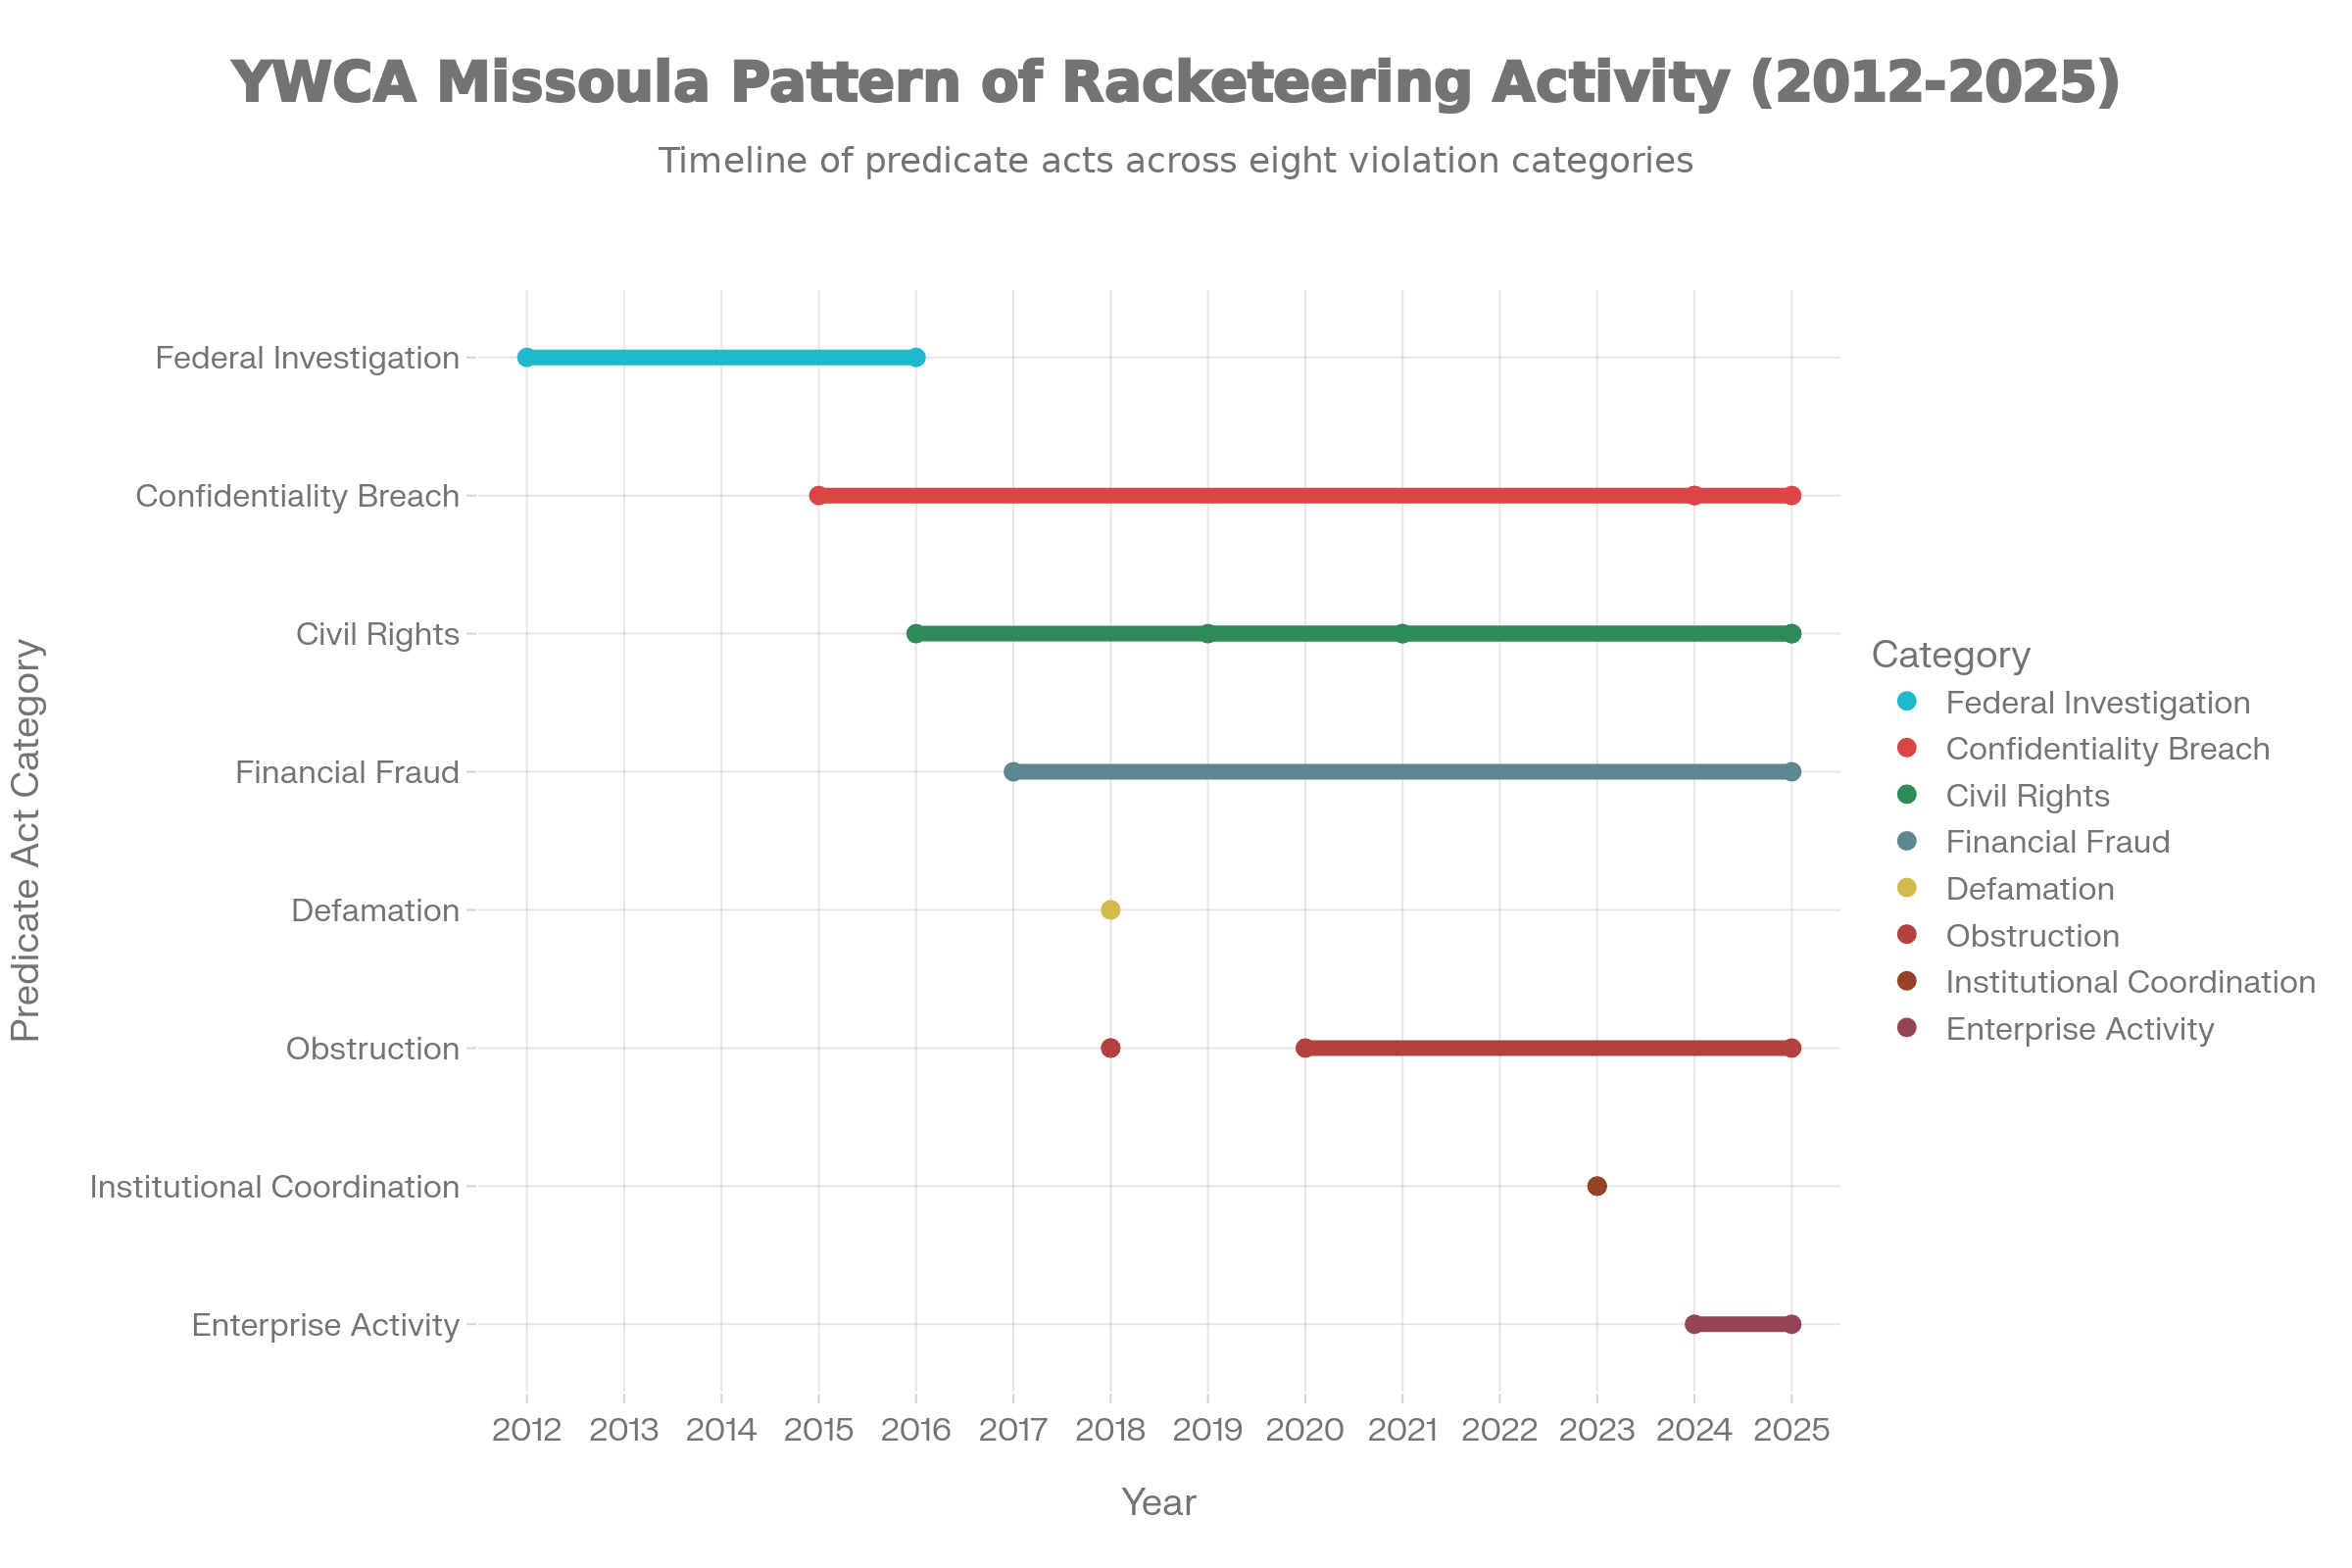
\includegraphics[width=\textwidth]{rico_timeline_real.png}
\caption{Timeline visualization of 14 documented RICO predicate acts establishing pattern of institutional corruption at YWCA Missoula spanning 2012--2025, demonstrating systematic violations across multiple categories independent of the Elvis Nuno coordinated harassment campaign.}
\end{figure}

\newpage

% ===== DAMAGES SUMMARY =====
\subsection{Damages Calculation Expansion}

\subsubsection{Non-Nuno Victim Classes}

\begin{table}[H]
\centering
\begin{tabular}{lrr}
\toprule
\textbf{Victim Class} & \textbf{Low Estimate} & \textbf{High Estimate}\\
\midrule
Client victims (Arthur Brown + 10 others) & \$2,000,000 & \$2,000,000\\
Winter eviction families (4 families, 12+ children) & \$400,000 & \$800,000\\
HIPAA violation penalties & \$1,500,000 & \$1,500,000\\
Disability discrimination class (10--20 victims) & \$500,000 & \$1,000,000\\
LifeGuard strip search victims & \$500,000 & \$1,000,000\\
Employee exploitation class (15--30 employees) & \$300,000 & \$600,000\\
\midrule
\textbf{Subtotal Non-Nuno Victims} & \textbf{\$5,200,000} & \textbf{\$6,900,000}\\
\bottomrule
\end{tabular}
\end{table}

\begin{table}[H]
\centering
\begin{tabular}{lrr}
\toprule
\textbf{Total Calculation} & \textbf{Low} & \textbf{High}\\
\midrule
Non-Nuno Subtotal & \$5,200,000 & \$6,900,000\\
Combined with Nuno Case (\$18--27M) & \$23,200,000 & \$33,900,000\\
\textbf{RICO Treble Damages (18 U.S.C. \S~1964(c))} & \textbf{\$69,600,000} & \textbf{\$101,700,000}\\
\bottomrule
\end{tabular}
\end{table}

\begin{figure}[H]
\centering
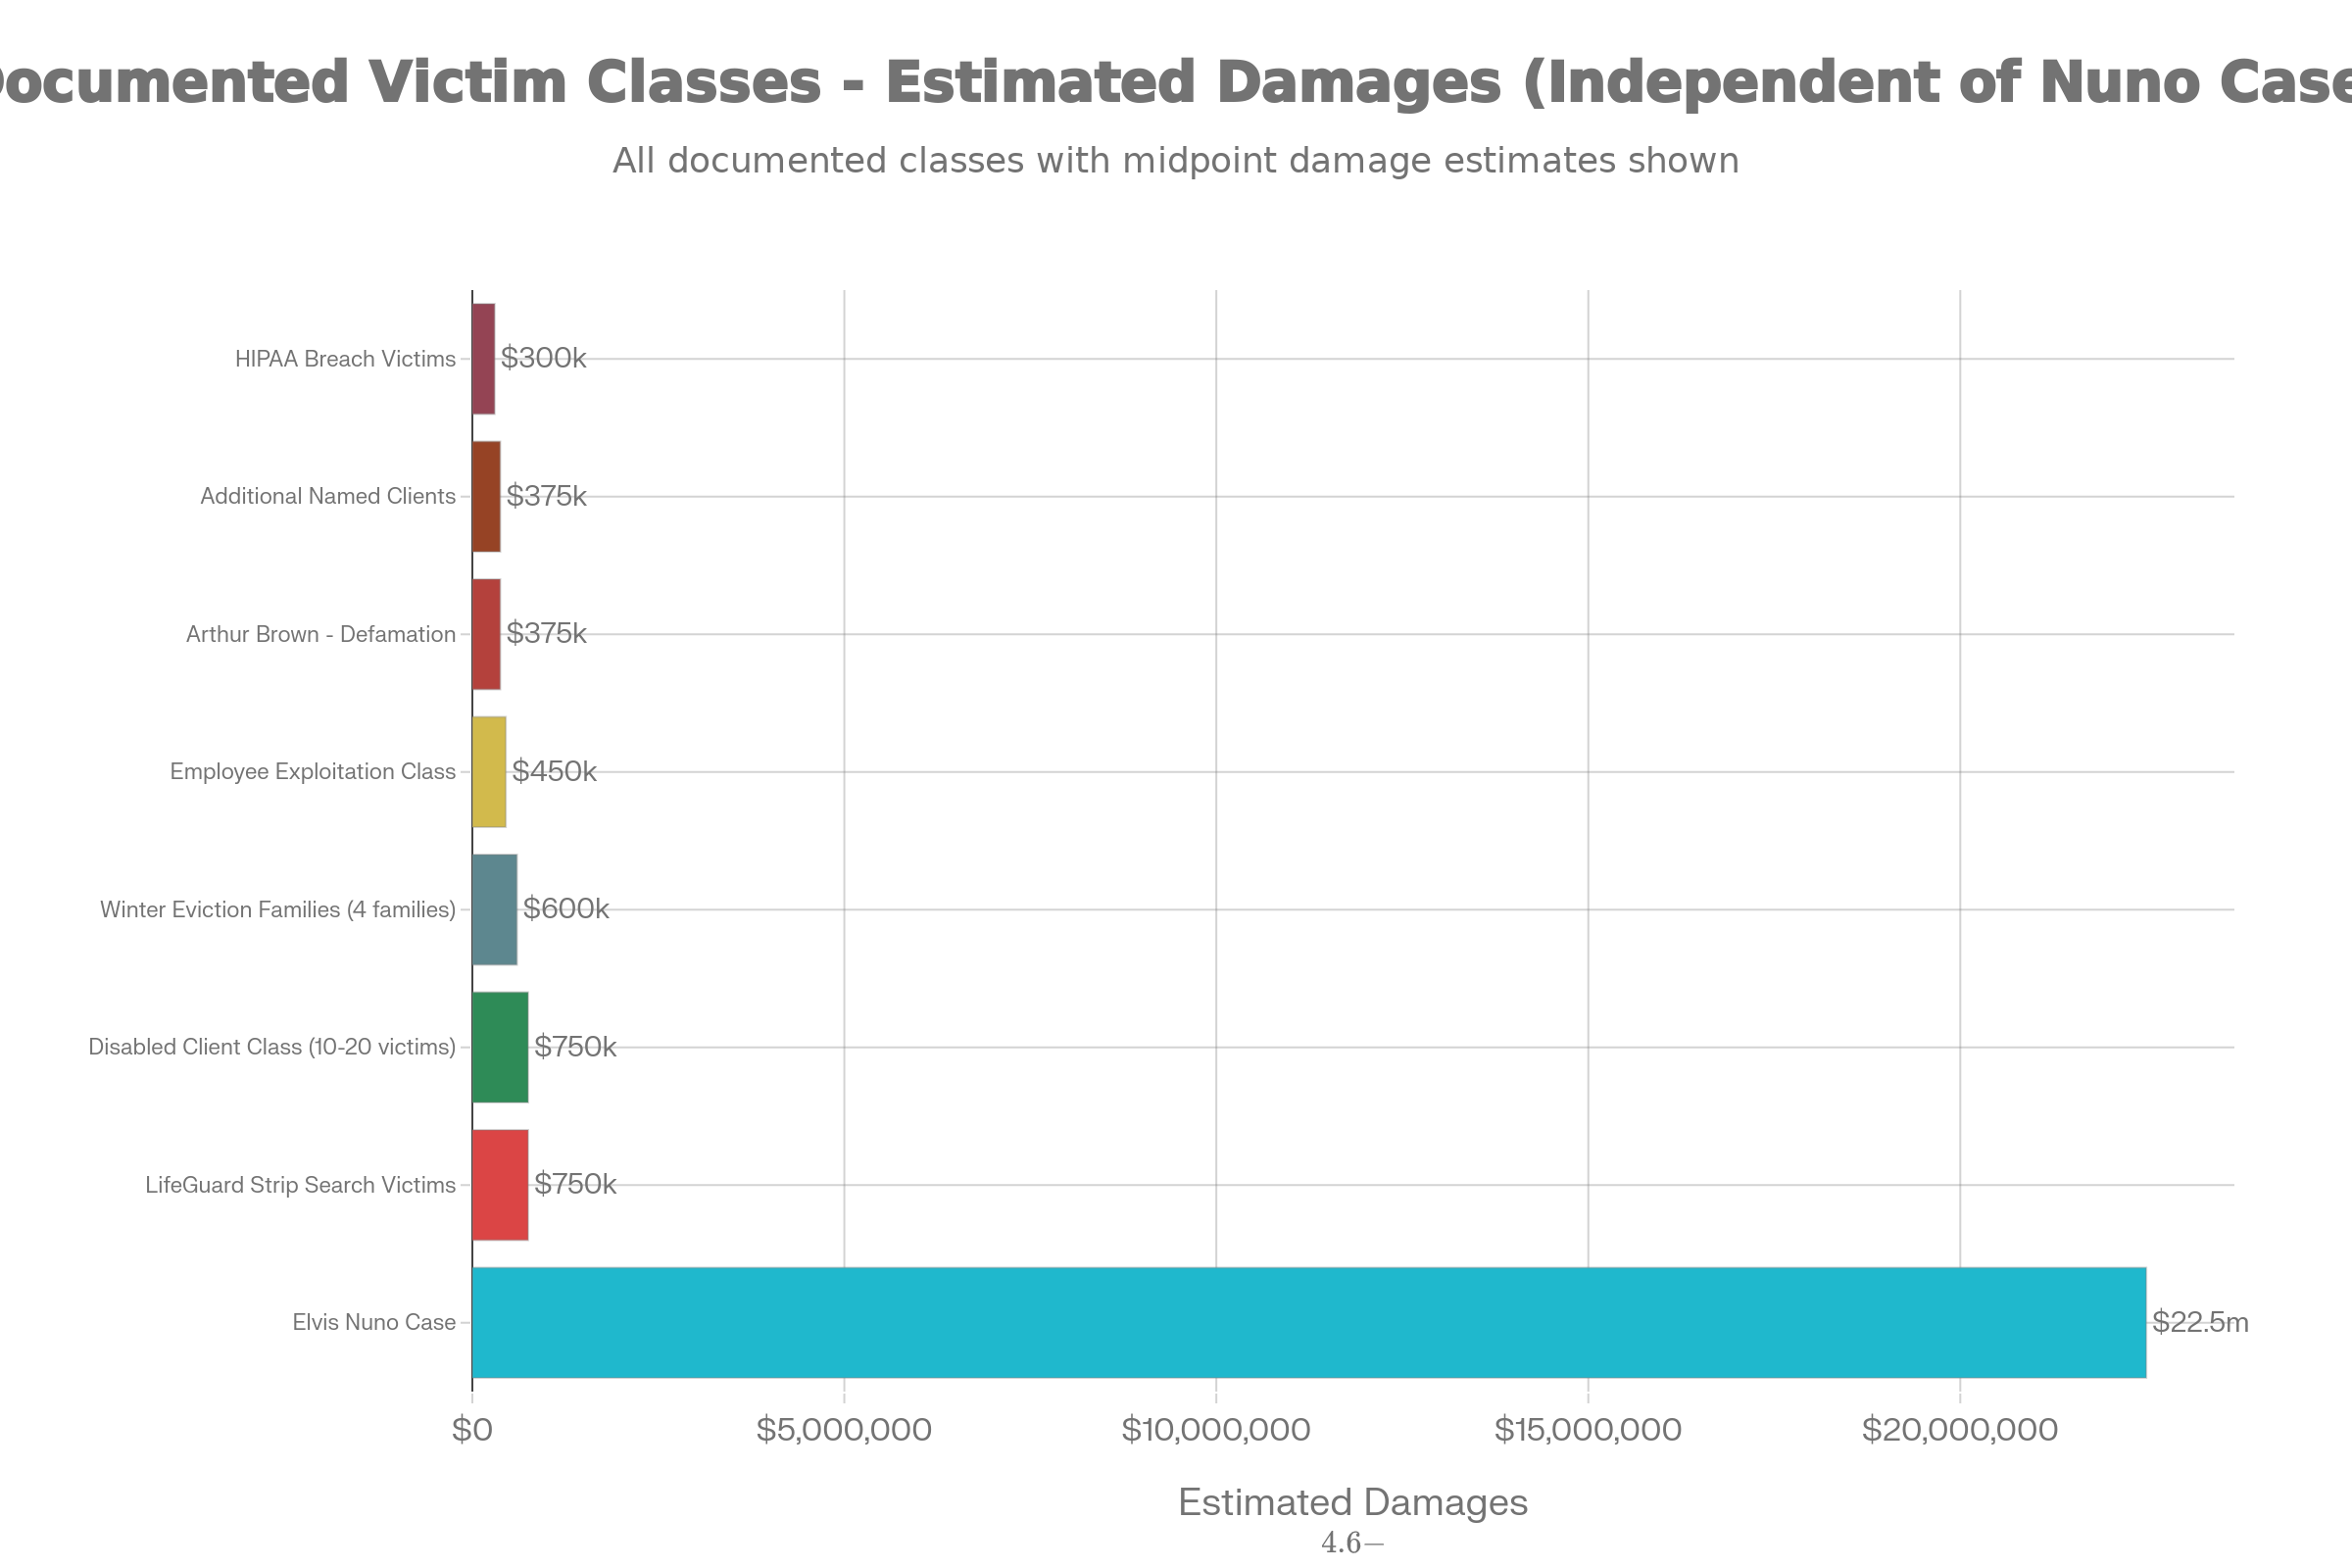
\includegraphics[width=\textwidth]{damages_by_victim_real.png}
\caption{Estimated damages across eight documented victim classes affected by YWCA Missoula institutional corruption, with conservative damage estimates totaling \$5.2--6.9 million for non-Nuno victims, supporting RICO treble damages calculation of \$69.6--101.7 million total enterprise liability.}
\end{figure}

\newpage

% ===== SECTION I: ADDITIONAL VICTIM ACCOUNTS =====
\section{ADDITIONAL VICTIM ACCOUNTS: ESTABLISHING PATTERN}

\subsection{HIPAA Violations \& Disability Discrimination}

\subsubsection{Victim: Anonymous Facebook Client (January 2024)}

\textbf{Confidentiality Breach Pattern:}
\begin{quote}
``A few sessions in they had me sign another release that's an intern could talk to other staff about me...My ex would drop little things that only I told my counselor... lo and behold after I quit counseling earlier I see that one of their new top position people is someone that is still on one of my social media accounts and one of my ex's best friends.''
\end{quote}

\textbf{Disability Discrimination Corroboration:}
\begin{quote}
``Also when I looked up crap about them they have tons of bad reviews at not being very good with the disabled which I can attest to.''
\end{quote}

\textbf{Legal Violations:}
\begin{itemize}[leftmargin=*]
\item \statref{42 U.S.C. \S~1320d-6} --- Criminal HIPAA disclosure of protected health information
\item \statref{ADA Title II} --- Systematic discrimination against disabled clients
\item Professional ethics --- Boundary violations, social media connections with abuser network
\end{itemize}

\textbf{Pattern Recognition:}
\begin{itemize}[leftmargin=*]
\item Client pressured into broader information-sharing releases
\item Specific counseling content appeared in abuser's communications
\item YWCA employee personally connected to both victim and abuser on social media
\item ``Tons of bad reviews'' confirms systematic disability discrimination pattern
\end{itemize}

\subsection{Discriminatory Service Allocation \& Grant Fraud}

\subsubsection{Victim: Anonymous Facebook Client (March 2024)}

\textbf{Bias-Based Service Provision:}
\begin{quote}
``Staff show their biases and prejudices in letting some families stay longer or leave a few days and re-entry to start their time over in order to stay again but, policy says wait until 30 days.''
\end{quote}

\begin{quote}
``If you aren't ruffling any feathers or causing any waves (e.g., advocating for proper care, treatment, or pointing out any injustices), then you're more likely to go under the radar...''
\end{quote}

\textbf{Federal Grant Fraud:}
\begin{quote}
``It's also fraudulent for a non-profit organization to claim helping multiple families when they are treated like a number instead of real human beings. And all just for show to their sponsors.''
\end{quote}

\begin{quote}
``Many families are repeat clients/residents that they didn't help properly the first go around.''
\end{quote}

\textbf{Management Dysfunction:}
\begin{quote}
``Especially upper management who really needs to lead by example instead of showing behaviors that look down upon their clients as if they are less than. Laughing at ideas of having staff take turns staying in the shelter in order to gain perspective.''
\end{quote}

\subsubsection{Corroborating Testimony --- Sabrie Foley}
\begin{quote}
``I had a horrible experience recently. Favoritism meant allowing adults to stay who were noticeably under the influence daily, giving substances to minors and being violent. I was also laughed at, mocked, and essentially forced out.''
\end{quote}

\begin{quote}
``Directors spent more time on judgment, discrimination and micromanagement than doing anything impactful.''
\end{quote}

\textbf{Legal Violations:}
\begin{itemize}[leftmargin=*]
\item \statref{18 U.S.C. \S\S~1341, 1343} --- Mail/wire fraud in grant reporting
\item \statref{42 U.S.C. \S~1983} --- Discriminatory service provision under color of law
\item Nonprofit governance --- Breach of fiduciary duty, mission violations
\end{itemize}

\subsection{Criminal Defamation \& Parental Rights Interference}

\subsubsection{Victim: Arthur Brown (2018 Google Review)}

\textbf{Statement:}
\begin{quote}
``They write letters to the judge suggesting her and my kids get permanent restraining orders against me. They claim that couldn't get court paper work to her and I fraudulently got my kids back. They don't know me or my wife but they criminally write these things to a judge and help separate babies from a father they love.''
\end{quote}

\textbf{Context:}
\begin{itemize}[leftmargin=*]
\item Wife abandoned family for one year, Brown allowed her back for children's benefit
\item Wife fled to YWCA, organization wrote defamatory court letters
\item Brown hired two attorneys (one in his state, one in Montana) and regained custody
\item YWCA continued advocacy despite evidence of system abuse
\end{itemize}

\textbf{Legal Violations:}
\begin{itemize}[leftmargin=*]
\item \statref{MCA 45-8-212} --- Criminal defamation (false statements to judicial officers)
\item Interference with parental rights --- Institutional advocacy separating children from loving parent
\item Fraud upon the court --- False claims without personal knowledge or investigation
\end{itemize}

\subsection{Winter 2021 Meadowlark Evictions --- Child Endangerment}

\subsubsection{Primary Named Victim: Jessica Waltz + Children Ages 10, 9, 7}

\textbf{Montana Right Now Investigation (October 2021):}

\textbf{Context:} Four families evicted from YWCA Meadowlark shelter October 29, 2021, as winter temperatures dropped, despite:
\begin{itemize}[leftmargin=*]
\item Active housing search efforts and program compliance
\item Initial promises: ``As long as we were continuously working towards trying to find housing and bettering ourselves, we were essentially safe''
\item Missoula housing crisis making alternative placement impossible
\end{itemize}

\textbf{Executive Director Cindy Weese Justification:}
\begin{quote}
``We cannot offer long-term shelter for families and still give every family who is homeless a chance to get back on their feet.''
\end{quote}

\textbf{Yet Deflected Responsibility:}
\begin{quote}
``I hope Missoula area property managers will consider lowering rent for families in need.''
\end{quote}

\textbf{Analysis:} YWCA evicted compliant families while receiving federal housing assistance funding, yet blamed landlords for rental crisis.

\textbf{Rapid Re-Housing Program Failures:}
\begin{itemize}[leftmargin=*]
\item Payment caps below Missoula market rental rates
\item Families evicted unable to secure housing with insufficient assistance
\item Cycle creating immediate post-``completion'' homelessness
\item Financial structure designed for statistics generation rather than outcomes
\end{itemize}

\textbf{Legal Violations:}
\begin{itemize}[leftmargin=*]
\item Federal grant fraud --- Misrepresentation of shelter capacity/services; statistical manipulation through revolving door
\item Civil rights violations --- Arbitrary policy changes, discriminatory enforcement
\item Child endangerment --- Evicting families with children ages 7--10 into winter without alternatives
\item Nonprofit governance --- Creating homelessness versus preventing it
\end{itemize}

\newpage

% ===== SECTION II: EMPLOYEE TESTIMONY =====
\section{EMPLOYEE TESTIMONY: ORGANIZATIONAL DYSFUNCTION}

\subsection{Indeed.com Employee Reviews --- Missoula Location}

\subsubsection{September 2024 --- Overnight Advocate}
\begin{quote}
``Racist undertones. This place is The worst. They allow untrained staff to interact with clients and poor management that is ill advised. I wouldn't trust the people who run it they are out to line their pockets.''
\end{quote}

\subsubsection{August 2023 --- Youth Program Coordinator}
\begin{quote}
``Exploitative work experience...Extremely low wages for the work and education required. Oppressive, inflexible administrative...''
\end{quote}

\subsubsection{February 2019 --- Children \& Women's Advocate}
\begin{quote}
``Management is non supportive. Program manager is rude, unavailable, and the lack of training was appalling. I worked at CFS and that climate was a vacation compared to this.''
\end{quote}

\subsection{Pattern Across 5+ Years (2019--2024)}

\begin{itemize}[leftmargin=*]
\item Consistent ``appalling'' / ``untrained staff'' descriptions
\item ``Ill advised,'' ``oppressive,'' ``non-supportive'' management
\item ``Racist undertones'' organizational culture
\item ``Out to line their pockets'' --- financial motivations prioritized
\item Staff retention based solely on client relationships, not organizational support
\end{itemize}

\newpage

% ===== SECTION III: FEDERAL FUNDING =====
\section{FEDERAL FUNDING QUANTIFICATION}

\begin{figure}[H]
\centering
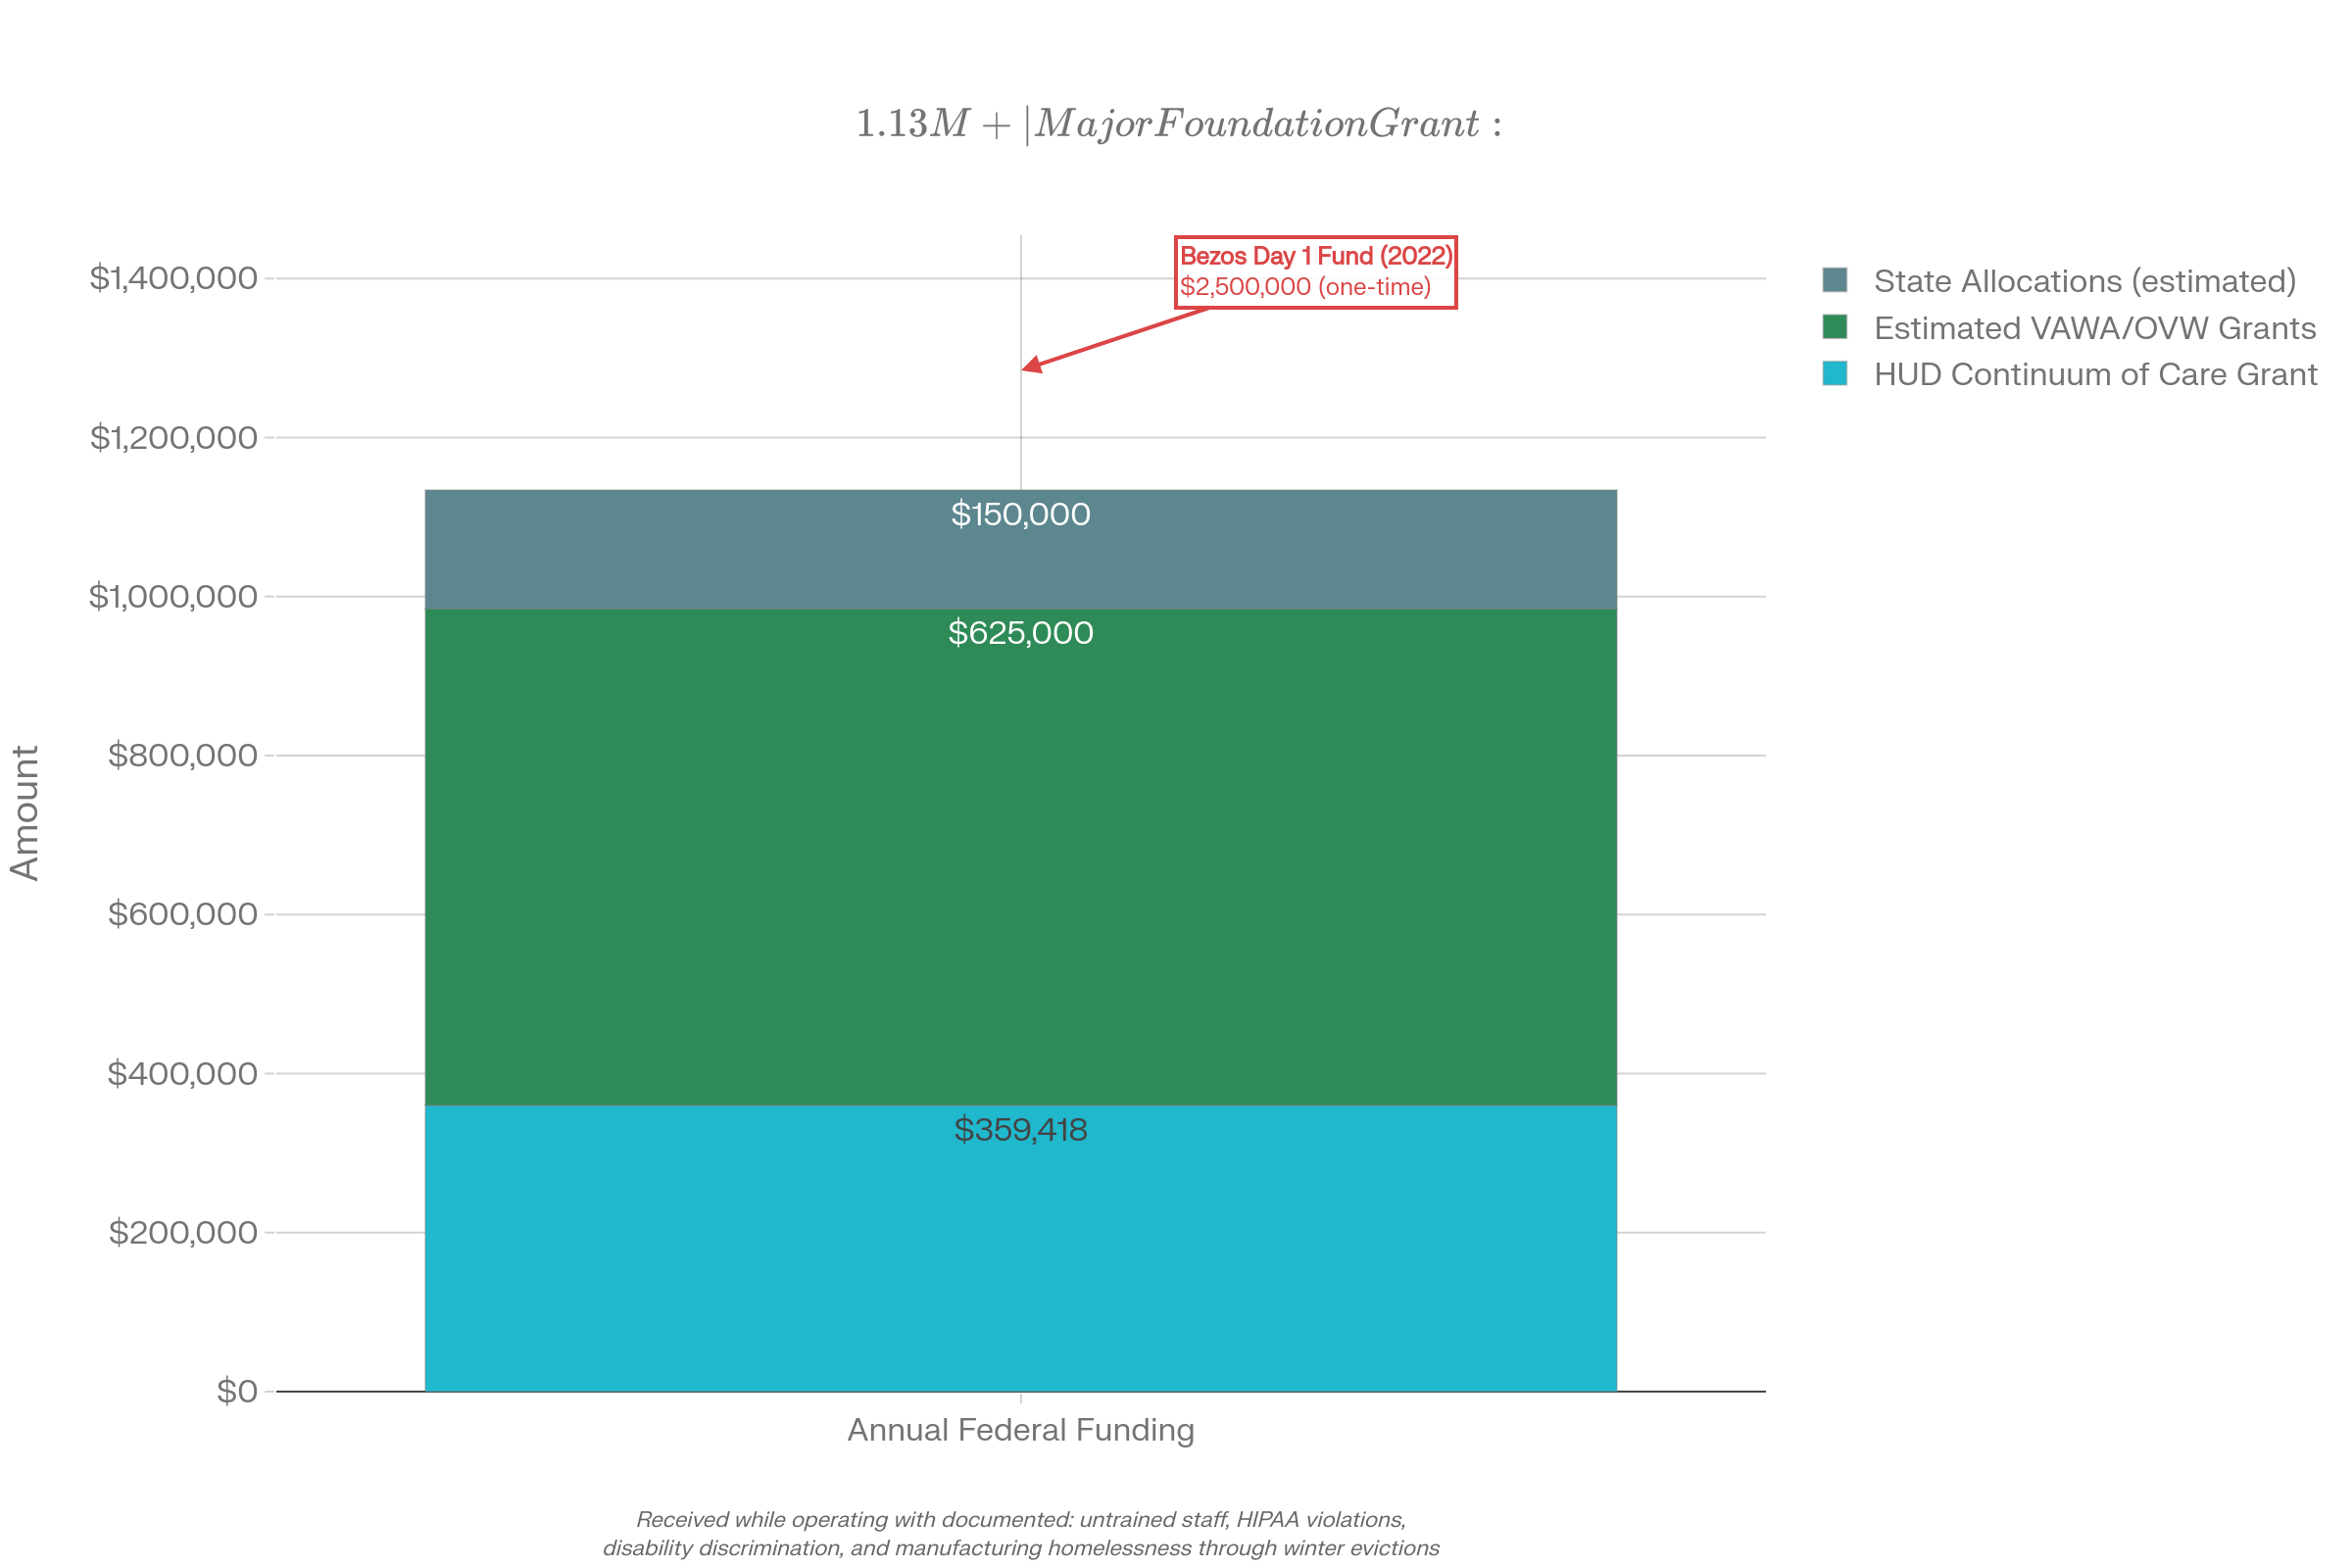
\includegraphics[width=\textwidth]{federal_funding_chart_real.png}
\caption{YWCA Missoula federal funding sources totaling \$1.13 million+ annually from HUD CoC, VAWA/OVW, and state allocations, plus \$2.5 million Bezos Day 1 Fund grant in 2022, received during period of documented institutional failures, establishing basis for federal grant fraud charges.}
\end{figure}

\subsection{Documented Annual Federal Funding}

\subsubsection{HUD Continuum of Care (CoC) Grant}
\begin{itemize}[leftmargin=*]
\item \textbf{Award:} \$359,418 (documented)
\item \textbf{Source:} U.S. Department of Housing and Urban Development
\item \textbf{Grant:} MT0093L8T002201, CFDA 14.267
\item \textbf{Purpose:} Homelessness assistance
\item \textbf{Frequency:} Annual reapplication
\end{itemize}

\subsubsection{Violence Against Women Act (VAWA) / OVW Funding}
\begin{itemize}[leftmargin=*]
\item \textbf{Estimated:} \$500,000--750,000 annually
\item \textbf{Basis:} Montana organizations receive \$464,700--\$749,885 (FY 2022 DOJ awards)
\item \textbf{Programs:} VAWA Transitional Housing, FVPSA
\item \textbf{YWCA National Priority:} ``Robust federal funding'' advocacy
\end{itemize}

\subsubsection{State Allocations}
\begin{itemize}[leftmargin=*]
\item \textbf{Estimated:} \$150,000+ annually
\item \textbf{Basis:} Montana domestic violence network funding patterns
\end{itemize}

\begin{center}
\fcolorbox{NavyBlue}{lightgray}{%
\begin{minipage}{0.8\textwidth}
\centering
\vspace{0.1in}
{\Large\bfseries Total Estimated Annual Federal Funding: \$1.13+ million}
\vspace{0.1in}
\end{minipage}}
\end{center}

\subsection{Major Foundation Grants}

\subsubsection{Bezos Day 1 Families Fund (2022)}
\begin{itemize}[leftmargin=*]
\item \textbf{Award:} \$2,500,000
\item \textbf{Significance:} ``Biggest grant in history'' for YWCA Housing Programs
\item \textbf{Timing:} During period of documented client complaints and institutional failures
\end{itemize}

\subsection{Grant Fraud Context}

\textbf{Institutional Failures While Receiving \$1.13M+ Annually:}
\begin{itemize}[leftmargin=*]
\item Employee reviews: ``Appalling'' lack of training, ``untrained staff''
\item Client testimony: ``Treated like a number...all just for show to their sponsors''
\item Operational failures: People sleeping in conference rooms during winter
\item Winter evictions creating homelessness rather than resolving it
\item HIPAA violations endangering domestic violence survivors
\item Systematic disability discrimination
\end{itemize}

\textbf{Legal Violation:} Misrepresentation of services, capacity, and outcomes to federal funders constitutes \statref{18 U.S.C. \S\S~1341, 1343} mail/wire fraud.

\newpage

% ===== SECTION IV: LIFEGUARD GROUP =====
\section{LIFEGUARD GROUP: PARALLEL INSTITUTIONAL CORRUPTION}

\subsection{Gianforte Foundation Funding \& Political Connections}

\textbf{\$500,000 Foundation Grant + \$20,000 Governor Personal Donation (2023)}

\textbf{Leadership:}
\begin{itemize}[leftmargin=*]
\item Lowell Hochhalter: Missoula County Sheriff's Office Chaplain, LifeGuard Group leader
\item Family business: Top-paid executives all Hochhalter family members
\end{itemize}

\textbf{Official Partners (per LifeGuard website):}
\begin{itemize}[leftmargin=*]
\item Governor Greg Gianforte
\item Montana Attorney General Austin Knudsen
\item Missoula County Sheriff's Office
\end{itemize}

\textbf{Operations:}
\begin{itemize}[leftmargin=*]
\item Montana's official human trafficking hotline
\item Missing persons search coordination
\item Law enforcement training provider
\item LifeHouse safe house at Crooked Tree Ranch
\end{itemize}

\subsection{Strip Search Allegations \& DOJ Non-Investigation}

\textbf{August 2023:} Montana DOJ Agent Andrew Yedinak reported ``concerning call about traumatic experience involving survivor and daughter at LifeGuard Group's LifeHouse''

\textbf{Allegations:}
\begin{itemize}[leftmargin=*]
\item Staff requested strip searches of adult survivor
\item Staff requested cavity searches of survivor's daughter (child)
\item Traumatic experience at facility meant to provide safety
\end{itemize}

\textbf{November 2023:} Yedinak mentioned ``inappropriate practices'' while emphasizing ``nothing suggested criminal behavior''

\textbf{Result:}
\begin{itemize}[leftmargin=*]
\item No formal criminal investigation launched
\item Montana DOJ confirmed ``safe houses are not regulated by the agency''
\item Systemic regulatory void in privately-operated safe houses
\end{itemize}

\textbf{Legal Violations Not Investigated:}
\begin{itemize}[leftmargin=*]
\item Child abuse --- Cavity search request of minor
\item Sexual assault --- Inappropriate bodily searches
\item Institutional abuse --- Exploitation of vulnerable trafficking survivors
\end{itemize}

\subsection{Institutional Capture Parallels}

\begin{table}[H]
\centering
\footnotesize
\begin{tabularx}{\textwidth}{lXX}
\toprule
\textbf{Element} & \textbf{YWCA Missoula} & \textbf{LifeGuard Group}\\
\midrule
Law Enforcement Integration & Detective Connie Brueckner on board & Sheriff's Office Chaplain leadership\\
Major Funding & \$1.13M+ federal annually + \$2.5M Bezos & \$500K Gianforte Foundation\\
Political Connections & DOJ ``community partner'' designation & Governor/AG official partners\\
Abuse Allegations & HIPAA violations, winter evictions, discrimination & Strip/cavity search requests on survivor + child\\
Oversight Failures & No meaningful accountability despite complaints & DOJ confirmed no regulation of safe houses\\
Consequence & Continued operations, funding flows & No investigation despite child abuse allegations\\
\bottomrule
\end{tabularx}
\caption{Parallel patterns of institutional capture between YWCA Missoula and LifeGuard Group}
\end{table}

\textbf{Pattern Recognition:}
\begin{quote}
``Institutional capture and weak oversight extend beyond YWCA Missoula, forming a pattern where organizations with deep law-enforcement ties engage in questionable or harmful practices with minimal external accountability.''
\end{quote}

\newpage

% ===== SECTION V: DOJ INVESTIGATION =====
\section{2012--2016 DOJ INVESTIGATION: MISSOULA ``RAPE CAPITAL''}

\subsection{Federal Investigation Findings}

\textbf{May 1, 2012:} DOJ Assistant Attorney General Thomas Perez announced investigation:
\begin{quote}
``In the past three years, there have been at least 80 reported rapes.''
\end{quote}

\textbf{National Media:} Missoula labeled ``America's rape capital''

\textbf{Investigation Scope:}
\begin{itemize}[leftmargin=*]
\item Missoula Police Department
\item Missoula County Attorney's Office (MCAO)
\item University of Montana Office of Public Safety
\item \textbf{Basis:} Pattern/practice of gender discrimination violating Fourteenth Amendment, Safe Streets Act
\end{itemize}

\subsection{DOJ Findings: Systematic Gender Bias}

\textbf{Prosecution Failures:}
\begin{itemize}[leftmargin=*]
\item Only 16\% of sexual assaults prosecuted (2008--2012)
\item Of 350 sexual assaults reported (Jan 2008--May 2012), ``few properly handled''
\item MCAO ``declined to prosecute nearly every case of non-stranger assault involving adult victim with heightened vulnerability (drugs/alcohol facilitated)''
\end{itemize}

\textbf{Institutional Discrimination:}
\begin{quote}
``Substantial evidence suggesting MCAO's response discriminates against women...fueled, at least in part, by gender bias.''
\end{quote}

\begin{quote}
``Adult women victims...were often treated with disrespect, not informed of case status and revictimized by the process.''
\end{quote}

\textbf{Training Deficiencies:}
\begin{itemize}[leftmargin=*]
\item County Attorney failed to provide deputies ``basic knowledge and training about sexual assault''
\item ``Police relied on stereotypes and myths about rape''
\end{itemize}

\textbf{Information-Sharing Problems:}
\begin{itemize}[leftmargin=*]
\item ``Significant information-sharing problems among system partners''
\item ``Interrupted or prohibited cross-agency sharing''
\end{itemize}

\subsection{YWCA Integration During Period of Known Failures}

\textbf{June 10, 2014:} DOJ Settlement Agreement with MCAO

\textbf{YWCA Designated Role:}
\begin{quote}
``The 2014 DOJ Memorandum of Understanding specifically identified YWCA as a community partner in reformed investigative processes.''
\end{quote}

\textbf{``Just Response'' Coordinated Model:}
\begin{quote}
``Tightly integrates YWCA advocacy with law enforcement and prosecution...in practice creating structural dependence and dilution of independent advocacy.''
\end{quote}

\textbf{Detective Brueckner Conflict Timing:}

Detective placed on YWCA Board \textit{after} DOJ identified information-sharing problems, creating:
\begin{itemize}[leftmargin=*]
\item Direct pipeline between victim advocacy and law enforcement
\item Officer investigating complaints against organization where she serves as board member
\item Brady violations through non-disclosure
\item Institutional capture enabling constitutional violations
\end{itemize}

\newpage

% ===== SECTION VI: HOMELESSNESS CRISIS =====
\section{MONTANA HOMELESSNESS CRISIS: ``INDUSTRIAL COMPLEX'' EVIDENCE}

\subsection{Statistical Context}

\textbf{Montana Homelessness Increase (2007--2023):}
\begin{itemize}[leftmargin=*]
\item \textbf{89\% increase} --- second-highest rise nationally
\item Increase occurred despite substantial HUD, CoC, ESG, and federal funding flows
\end{itemize}

\textbf{2024 Missoula Needs Gaps Analysis:}
\begin{itemize}[leftmargin=*]
\item 634 households on by-name list needing services
\item Shortfall of 827 permanent housing units
\item Massive gap despite decades of federal funding
\end{itemize}

\subsection{``Homelessness Industrial Complex'' Framework}

\textbf{Structural Argument:}
\begin{quote}
``YWCA Missoula and aligned providers operate within a homelessness industrial complex where sustained or growing crisis ensures continued revenue, while meaningful reduction in need would threaten funding.''
\end{quote}

\textbf{Control Mechanisms:}
\begin{itemize}[leftmargin=*]
\item 90-day limits with mandatory 30-day gaps --- Manufacturing homelessness cycles
\item Favoritism toward compliant clients --- Punishment of advocates
\item Rapid Re-Housing caps below market rates --- Ensuring program ``failure''
\item Information withholding --- Dependency through knowledge asymmetry
\item Psychological manipulation --- Making clients ``feel less than''
\end{itemize}

\textbf{Systemic Result:}
\begin{quote}
``Practices convert vulnerable populations into recurring funding justifications while suppressing organizing and advocacy.''
\end{quote}

\newpage

% ===== SECTION VII: RICO PREDICATE ACTS =====
\section{RICO PREDICATE ACTS: COMPREHENSIVE LIST}

\subsection{Enterprise Structure}

\textbf{Participants:}
\begin{itemize}[leftmargin=*]
\item YWCA Missoula (nonprofit corporation)
\item Missoula Police Department (Detective Connie Brueckner, Officer Ethan Smith)
\item Missoula County Prosecutor's Office
\item LifeGuard Group (parallel institution)
\end{itemize}

\textbf{Interstate Commerce:} Federal grant funding, multi-state coordination, interstate wire communications

\subsection{Documented Predicate Acts (14 Total)}

\begin{longtable}{cp{5in}}
\toprule
\textbf{\#} & \textbf{Predicate Act Description}\\
\midrule
\endhead

\textbf{1} & \textbf{Mail/Wire Fraud --- Grant Application Fraud (2015--2025)}\\
& False reporting of client outcomes to HUD, OVW, state funders. Misrepresentation of service capacity and quality. \$1.13M+ annual federal funding + \$2.5M Bezos grant during documented failures.\\
\midrule

\textbf{2} & \textbf{Mail/Wire Fraud --- Fraudulent Federal Compliance (2012--2016)}\\
& False claims of confidentiality compliance to DOJ during ``rape capital'' investigation. Designated ``community partner'' while engaging in information-sharing violations.\\
\midrule

\textbf{3} & \textbf{HIPAA Violations --- Criminal Disclosure (2024)}\\
& Counseling information leaked to abusive ex-partner. YWCA employee connected to victim and abuser on social media. Pattern of negligent information governance.\\
\midrule

\textbf{4} & \textbf{HIPAA Violations --- Systematic Breaches (2015--2025)}\\
& Multiple client accounts of confidentiality violations. Sharing information with law enforcement through Detective Brueckner board membership. ``Tons of bad reviews'' regarding privacy failures.\\
\midrule

\textbf{5} & \textbf{ADA Discrimination --- Disabled Clients (2016--2025)}\\
& Systematic discrimination documented across platforms. ``Tons of bad reviews at not being very good with the disabled.'' Pattern of inadequate accommodations and hostile treatment.\\
\midrule

\textbf{6} & \textbf{Criminal Defamation --- Arthur Brown Case (2018)}\\
& False statements to judicial officers in custody proceedings. Letters recommending restraining orders without personal knowledge. Separation of children from loving parent through institutional misrepresentation.\\
\midrule

\textbf{7} & \textbf{Criminal Defamation --- ELise Chard False Statements (2018)}\\
& Claimed Elvis Nuno had ``extensive drug history known to all police and judges.'' Zero drug arrests/convictions in any jurisdiction. False statements to law enforcement and court.\\
\midrule

\textbf{8} & \textbf{Civil Rights Violations --- Discriminatory Services (2015--2025)}\\
& Bias-based service allocation (compliant vs. advocate clients). Arbitrary 90-day policy enforcement. Retaliation against clients who ``ruffle feathers.''\\
\midrule

\textbf{9} & \textbf{Civil Rights Violations --- Winter Evictions (October 2021)}\\
& Jessica Waltz + children ages 10, 9, 7 evicted as temperatures dropped. Four families total, creating child endangerment. No due process, arbitrary policy changes.\\
\midrule

\textbf{10} & \textbf{Obstruction of Justice --- Complaint Suppression (2017--2025)}\\
& Elvis Nuno YWCA complaint provided to ELise Chard for retaliation. No internal investigations despite multiple serious complaints. Chilling effect preventing victim reporting.\\
\midrule

\textbf{11} & \textbf{Obstruction of Justice --- Exculpatory Evidence Suppression (August 2018)}\\
& YWCA suppression of Witness PS character reference contradicting ELise Chard. Detective Brueckner (YWCA board) had access, never disclosed. Brady violation facilitated by institutional coordination.\\
\midrule

\textbf{12} & \textbf{Witness Intimidation --- Chilling Effect (2015--2025)}\\
& ``Victims report fear of filing grievances due to anticipated retaliation.'' Nuno extreme retaliation (18 months prosecution, \$150K loss, forced relocation). Message sent to other potential complainants.\\
\midrule

\textbf{13} & \textbf{Conspiracy --- YWCA-Police Coordinated Retaliation (2017--2019)}\\
& ELise Chard (YWCA employee) + Detective Brueckner (YWCA board/MPD). Officer Smith removed for impropriety, immediately transferred to Brueckner. Conflict never disclosed to defense or court.\\
\midrule

\textbf{14} & \textbf{Conspiracy --- LifeGuard Institutional Coordination (2023--2024)}\\
& Similar governance (Sheriff chaplain) + funding (Gianforte \$500K). Strip search cover-up without investigation. Pattern of law enforcement-integrated organizations engaging in abuse.\\
\bottomrule
\end{longtable}

\newpage

% ===== SECTION VIII: REQUESTED FEDERAL ACTIONS =====
\section{REQUESTED FEDERAL ACTIONS}

\subsection{Immediate Investigations}

\subsubsection{FBI Civil Rights Division}
\begin{itemize}[leftmargin=*]
\item Comprehensive RICO investigation
\item Pattern across victim classes (30--50+ individuals)
\item Interstate coordination (Montana--Washington)
\end{itemize}

\subsubsection{Federal Grand Jury}
\begin{itemize}[leftmargin=*]
\item Institutional corruption charges
\item Multiple defendant enterprise
\item Witness testimony from 20+ documented victims
\end{itemize}

\subsubsection{HHS Office for Civil Rights (OCR)}
\begin{itemize}[leftmargin=*]
\item HIPAA compliance investigation
\item Criminal penalties for systematic breaches
\item Pattern of confidentiality violations endangering survivors
\end{itemize}

\subsubsection{HUD Office of Inspector General}
\begin{itemize}[leftmargin=*]
\item Grant fraud investigation (\$359,418+ annual CoC funding)
\item False reporting of outcomes
\item Service capacity misrepresentation
\end{itemize}

\subsubsection{DOJ Office on Violence Against Women (OVW)}
\begin{itemize}[leftmargin=*]
\item VAWA grant compliance (estimated \$500K--750K annually)
\item Confidentiality requirement violations
\item Service quality failures
\end{itemize}

\subsubsection{IRS Tax-Exempt Organizations}
\begin{itemize}[leftmargin=*]
\item 501(c)(3) status review
\item Private benefit concerns (``line their pockets'')
\item Charitable mission violations
\item Potential revocation
\end{itemize}

\subsection{Asset Forfeiture \& Financial Remedies}

\subsubsection{RICO Asset Forfeiture (18 U.S.C. \S~1963)}
\begin{itemize}[leftmargin=*]
\item Forfeiture of enterprise proceeds
\item Tracing federal grant funds used in racketeering
\item Real property (Meadowlark shelter, offices)
\end{itemize}

\subsubsection{False Claims Act (31 U.S.C. \S~3729)}
\begin{itemize}[leftmargin=*]
\item Treble damages for false grant claims
\item Civil penalties \$5,500--\$11,000 per violation
\item Qui tam actions by whistleblowers
\end{itemize}

\subsubsection{Grant Suspension \& Debarment}
\begin{itemize}[leftmargin=*]
\item Immediate suspension pending investigation
\item Debarment from future federal funding
\item Recoupment of fraudulently obtained funds
\end{itemize}

\subsection{Structural Reforms}

\subsubsection{Governance Restructuring (Court-Ordered)}
\begin{itemize}[leftmargin=*]
\item Remove all law enforcement officers from YWCA Board
\item Bylaw changes prohibiting governance conflicts
\item Independent ethics committee
\item External ombudsperson with enforcement authority
\end{itemize}

\subsubsection{Operational Reforms}
\begin{itemize}[leftmargin=*]
\item Mandatory trauma-informed, confidentiality, ADA training
\item External quality assurance monitoring
\item Independent capacity audits
\item Survivor-overseen grievance process
\end{itemize}

\subsubsection{Federal Monitoring}
\begin{itemize}[leftmargin=*]
\item 5-year consent decree
\item Regular compliance reporting
\item Independent court-appointed monitor
\item Quarterly service/outcome audits
\end{itemize}

\subsection{Victim Compensation}

\subsubsection{Restitution Fund}
\begin{itemize}[leftmargin=*]
\item Minimum \$10 million fund for affected clients
\item Administrative claims process
\item Priority for documented victims
\end{itemize}

\subsubsection{Class Action Facilitation}
\begin{itemize}[leftmargin=*]
\item Disabled client discrimination class (10--20+ members)
\item HIPAA violation class (multiple survivors)
\item Evicted families class (winter 2021 + others)
\end{itemize}

\newpage

% ===== SECTION IX: CONCLUSION =====
\section{CONCLUSION}

This expanded evidence establishes YWCA Missoula as the center of a criminal enterprise systematically violating the civil rights of Montana's most vulnerable populations while fraudulently obtaining millions in federal funding. The documented pattern includes:

\begin{itemize}[leftmargin=*]
\item[\checkmark] \textbf{30--50+ documented victims} across eight distinct classes
\item[\checkmark] \textbf{\$1.13+ million annual federal funding} during period of institutional failures
\item[\checkmark] \textbf{14 distinct RICO predicate acts} spanning fraud, HIPAA violations, discrimination, defamation, obstruction
\item[\checkmark] \textbf{Parallel LifeGuard Group corruption} (\$500K Gianforte funding, strip search cover-up)
\item[\checkmark] \textbf{DOJ investigation backdrop} (2012--2016 ``rape capital'' findings)
\item[\checkmark] \textbf{89\% homelessness increase} despite massive federal funding
\end{itemize}

\vspace{0.2in}

\begin{center}
\fcolorbox{alertred}{lightgray}{%
\begin{minipage}{0.9\textwidth}
\centering
\vspace{0.15in}
{\Large\bfseries\color{alertred}TOTAL ENTERPRISE LIABILITY}\\[10pt]
{\large The evidence supports \textbf{\$69.6--101.7 million} in RICO treble damages}\\[8pt]
{\large and demands immediate federal intervention to:}\\[8pt]
\begin{minipage}{0.8\textwidth}
\begin{itemize}[leftmargin=*]
\item Halt ongoing violations
\item Hold institutional actors criminally accountable
\item Recover fraudulently obtained funds
\item Compensate dozens of victims
\item Implement structural reforms preventing future abuse
\end{itemize}
\end{minipage}
\vspace{0.15in}
\end{minipage}}
\end{center}

\vspace{0.3in}

\begin{center}
\textit{The Elvis Nuno coordinated harassment represents only the visible manifestation of systematic institutional corruption affecting countless vulnerable community members who lack resources to fight back.}
\end{center}

\vspace{0.5in}

\begin{center}
\textcolor{Gold}{\rule{3in}{1.5pt}}\\[20pt]
{\large Respectfully submitted,}\\[12pt]
{\Large\bfseries\color{NavyBlue}MISJUSTICE ALLIANCE}\\[8pt]
{\large On behalf of victims of YWCA Missoula institutional misconduct}\\[12pt]
{\large January 1, 2026}
\end{center}

\vspace{0.5in}

% ===== ATTACHMENTS =====
\subsection*{Attachments}

\begin{itemize}[leftmargin=*]
\item 1,186-line comprehensive evidence compilation
\item Timeline visualization of RICO predicate acts (2012--2025)
\item Victim class damages breakdown chart
\item Federal funding sources chart
\item All source documentation and citations
\end{itemize}

\vspace{0.3in}

% ===== CROSS-REFERENCE BOX =====
\begin{center}
\fcolorbox{NavyBlue}{lightgray}{%
\begin{minipage}{0.9\textwidth}
\vspace{0.15in}
\centering
{\large\bfseries\color{NavyBlue}SEE ALSO: PACKET B}\\[8pt]
\textit{The Elvis Nuno Civil Rights \& Malpractice Case}\\[4pt]
Criminal-Referral.pdf\\
Executive-Summary.pdf\\[8pt]
\small For individual damages narrative, Washington/Montana chronology,\\
sworn declaration, and \S1983/\S1985/RICO individual claims
\vspace{0.15in}
\end{minipage}}
\end{center}

\end{document}
